\begin{figure}[htb]
	\begin{center}
		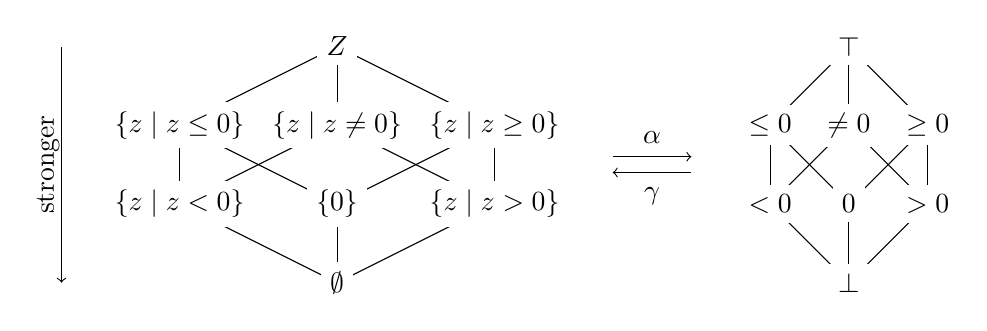
\begin{tikzpicture}
			% Concrete domain
			\draw (-4.5,0) -- (-6.5,1);
            \draw (-4.5,0) -- (-4.5,1);
            \draw (-4.5,0) -- (-2.5,1);
            \draw (-4.5,3) -- (-6.5,2);
            \draw (-4.5,3) -- (-4.5,2);
            \draw (-4.5,3) -- (-2.5,2);
            
            \draw (-4.5,1) -- (-6.5,2);
            \draw (-4.5,1) -- (-2.5,2);
            \draw (-6.5,1) -- (-6.5,2);
            \draw (-2.5,1) -- (-2.5,2);
            \draw (-4.5,2) -- (-6.5,1);
            \draw (-4.5,2) -- (-2.5,1);
            
            \draw (-4.5,0) node[fill=white!5] {$\emptyset$};
            \draw (-6.5,1) node[fill=white!5] {$\{z\;|\;z<0\}$};
            \draw (-4.5,1) node[fill=white!5] {$\{0\}$};
            \draw (-2.5,1) node[fill=white!5] {$\{z\;|\;z>0\}$};
            \draw (-6.5,2) node[fill=white!5] {$\{z\;|\;z\leq0\}$};
            \draw (-4.5,2) node[fill=white!5] {$\{z\;|\;z\neq0\}$};
            \draw (-2.5,2) node[fill=white!5] {$\{z\;|\;z\geq0\}$};
            \draw (-4.5,3) node[fill=white!5] {$\mathbb{Z}$};

			% Abstract domain
            \draw (2,0) -- (1,1);
            \draw (2,0) -- (2,1);
            \draw (2,0) -- (3,1);
            \draw (2,3) -- (1,2);
            \draw (2,3) -- (2,2);
            \draw (2,3) -- (3,2);
            
            \draw (2,1) -- (1,2);
            \draw (2,1) -- (3,2);
            \draw (1,1) -- (1,2);
            \draw (3,1) -- (3,2);
            \draw (2,2) -- (1,1);
            \draw (2,2) -- (3,1);
            
            \draw (2,0) node[fill=white!5] {$\perp$};
            \draw (1,1) node[fill=white!5] {$<0$};
            \draw (2,1) node[fill=white!5] {$0$};
            \draw (3,1) node[fill=white!5] {$>0$};
            \draw (1,2) node[fill=white!5] {$\leq0$};
            \draw (2,2) node[fill=white!5] {$\neq0$};
            \draw (3,2) node[fill=white!5] {$\geq0$};
            \draw (2,3) node[fill=white!5] {$\top$};
            
            
            % Arrows
            \draw (-0.5,1.85) node {$\alpha$};
            \draw [->](-1,1.6) -- (0,1.6);
            \draw [<-](-1,1.4) -- (0,1.4);
            \draw (-0.5,1.1) node {$\gamma$};
            
            \draw [<-](-8,0) -- (-8,3);
            \draw (-8.17,1.5) node[rotate=90] {stronger};
        \end{tikzpicture}
        \caption{The sign properties of the concrete integer domain (left) next to the abstract sign domain (right) as a Hasse diagram. }
	\end{center}
\end{figure}